%
% Analysis and forecasting of the Swiss Rent Index
% 1993 to 2018
%
% authors:      Faralli Zully, Spörri Marc
% date-hand-in: 2018-05
%

\documentclass[11pt,a4paper]{article}

% Setup packages
% ------------------------------------------------------------------------

% set margins ect of page
\usepackage[
    a4paper,
    top=1in,
    bottom=1in,
    left=1in,
    right=1in
]{geometry}
% \usepackage{fullpage}  % don't use fullpage, use the more advanced geometry package

\usepackage[T1]{fontenc}
\usepackage[utf8]{inputenc} 

\usepackage[english]{babel}  % language settings
\usepackage{lmodern}         % font to use
\usepackage{chngcntr}        % to be able to change figure counters
\usepackage{makecell}        % make line breaks inside table cells

\usepackage{graphicx}        % use modern graphics formats

\usepackage{amsmath}         % math packages
\usepackage{amssymb}
\usepackage{siunitx}         % takes care of units and errors

\usepackage[round]{natbib}   % bibliography options

\usepackage{xcolor}          % use color names


% hyperref creates links in a pdf, and lets you set pdf options
\usepackage[
    pdfpagelabels,
    plainpages=false,
    pdfauthor={Faralli Zully, Spörri Marc},
    pdftitle={Analysis and forecasting of the Swiss Rent Index 1993 to 2018},
    pdfproducer={},
    pdfcreator={LaTeX2e (pdfLaTeX+Biber/Biblatex on Kile/TexLive/Debian9 and TeXnicCenter/MiKTeX2.9/Windows10)},
    pdfsubject={Analysis and forecasting of the Swiss Rent Index 1993 to 2018},
    pdfkeywords={swiss rent index}
]{hyperref}   % Hyperlinks

% clever refs lets you write just \cref{x} instead of figure~\ref{x}, section~\ref{y} ect..
\usepackage[
    %capitalise,   % cap the fig, table... refs
    noabbrev,     % use Figure instead of fig.
    nameinlink    % make the whole thing clickable
]{cleveref}


% Settings
% ------------------------------------------------------------------------

% fuer nicht eingerueckter Absatzbegin folgendes auskommentieren:
\setlength\parindent{0pt}    % laenge des absatzeinzuges festlegen

\counterwithin{figure}{section}  % include section number in figure numbering
\bibliographystyle{apa}      % bibliography style to use
\graphicspath{{graphics/}}   % all graphics are in the graphics folder.
                             % by default, search there!

% prevent empty pages with only one image by tweeking some parameters
\renewcommand{\topfraction}{.8}
\renewcommand{\floatpagefraction}{.8}  % if more than x % of a page is an image
                                       % it will be a single image page.
                             




% My own commands
% ------------------------------------------------------------------------

% note \TODO{} in teh sourcecode to get reminded later that you still have work todo
\newcommand{\TODO}[1]{%
    \textcolor{red}{ %
        \textbf{[ !!!TODO: #1 ]}%
    }%
    \PackageWarning{TODO:}{TODO: #1}%
}


% The actual document
% ------------------------------------------------------------------------
\begin{document}


% titlepage
% ------------------------------------------------------------------------

\thispagestyle{empty}  % no pagenumber on this page

\begin{center}

\vspace*{4cm}

\noindent\rule{15cm}{0.4pt}

\vspace*{2cm}

\Huge{\textbf{Analysis and Forecasting of the Swiss Rent Index, 1993 to 2018}}

\vspace{1cm}

\LARGE{Project in Time Series Analysis -- Spring 2018}

\vspace{2cm}

\noindent\rule{15cm}{0.4pt}

\vfill

\large{
    \today\\
    University of Neuchâtel\\
    Faralli Zully, Spörri Marc\\
    
}

\vspace{2cm}

\end{center}


\newpage



% TOC
% ------------------------------------------------------------------------

\tableofcontents
\newpage


% ------------------------------------------------------------------------

\section{Introduction}

In this project we analyze the time series of the quarterly collected Swiss rent index from 1993 to 2018.
The main goal of the project is to draw inference from the rent index time series and to predict its future values and a future trend.
In order to do that we do first a transformation of the data in a mean-centered stationary time series by eliminating the trend and possible seasonal components.
Afterwards we are going to model our transformed, stationary data by fitting and testing a set of autoregressive moving average processes (ARMA) in order to select the best candidate model for our transformed, stationary data \cite[p.~82--110]{bd02}.
The selected model will be used to describe and interpret our data as well as to predict future values for the Swiss rent index.


% ------------------------------------------------------------------------

\section{Data Description and Data Analysis}

The data is provided by the Swiss Federal Statistical Office, implying 100 quarterly observations of the Swiss rent index beginning by the 2nd quarter of the year 1993 and ending by the first quarter of the year 2018.
The rent index measures the inflation of the rented dwellings in Switzerland.
It is the most significant partial index of the Swiss consumer’s price index, representing a weighted share of 13 percent of this index.

\begin{figure} [ht]
    \centering
    \includegraphics[width=0.7\textwidth]{indiceloyers_timeseries}
    \caption{Swiss rent index, years 1993 to 2018}
    \label{fig:indiceloyers_timeseries}
\end{figure}

The data are collected quarterly, based upon a stratified random survey sampling of around \num{10000} lessors.
The time series' first observation (2nd quarter of the year 1993) will be the reference value which is set to a base index of 100 and represents the weighted average rent at this time in Switzerland (OFS, 2016: p. 20-23).\\
The first step in any analysis of a time series is to identify possible discontinuities or a sudden change of level in the series\cite[p.~23]{bd02}.
As we can see from \cref{fig:indiceloyers_timeseries} there seems to be a evidently positive monotonic trend in the time series of the Swiss rent index.
However, the increase seems to be higher in the 1990ies.\\
It may be advisable to analyse the series by  segments \cite[p.~23]{bd02}.
For that purpose we have a look at the segmented plots 1993 to 2009 and 2009 to 2018.
We can see a slightly slower increase in the period from 2009 to 2018 indicating that during the years 1993 to 2009 the growth in rents was faster than in the years after the year 2009.\\
This fact can be well explained by the big real estate depression in the early 90ies in Switzerland, therefore the time series starting at 1993 is consequently starting from a relatively low initial level and, given the low initial level and the better conjunctural perspectives, the growth  was faster during the 1990ies (irgendwas zitieren 90er jahre depression), whereas from the year 2009 on the growth in rents slowed down, which can be very well explained by the US subprime crises triggered in the year 2008 and followed by a long-lasting global recession \TODO{(zitiere irgendwas)}.

However, they are apparently no outliers, sudden changes or major discontinuities and there is evidently no reason to do further data adjustments or variance-stabilizing transformations like Box-Cox-transformations, for instance \citep{boxcox64}.
Therefore we start our work in the next section by transforming our data into a stationary time series \cite[p.~45--82]{bd02}.


% ------------------------------------------------------------------------

\section{Transformation of the Data into a Stationary Time Series}

In this section we want to produce a noise sequence with no apparent deviations from stationarity, meaning we want to transform our data in such a way that covariances between the observations are not depending on time and that we obtain a zero mean expectation and constant variances \cite[pp.~14--23]{bd02}.

However, the objective is not to get a pure white noise sequence  with no dependence among the residuals neither, since there would no further modelling to be done except to estimate their mean-expectation (which would be zero in the centered transformed series) and variance.
The objective is to obtain a stationary series with some few significant dependence among the residuals anyhow, so we can look for a more complex stationary time series model for the noise that accounts for the dependence.
Since dependence means that past observations of the noise sequence can assist in predicting future values this allows us to get a better prediction quality than with a pure white noise sequence \cite[p.~35]{bd02}.

In order to get our noise sequence we have to eliminate any trend and/or seasonal components from our data.
In the next few subsections we will fit several models to get a stationary series.\\
Afterwards we test our fitted models first for stationarity by tests like the Augmented Dickie-Fuller-Test for the null hypothesis of a unit root (with the alternative hypothesis of stationarity, by consequence \citep{adf}) \\

Furthermore we test the estimated noise sequences by examining some simple tests whether or not the obtained residuals are values of independent and identically distributed random variables (as mentioned above: that should not necessarily occur, otherwise we would be confronted with too much randomness in our stationary series and our prediction work would be simply done by estimating mean of the white-noise, which is zero for all predictions $X_{n+1}$, $X_{n+2}$, $X_{n+3}$ etc. in case of a mean-centered stationary series).

In a final step we check them visually by plotting the autocorrelation-function as well as the partial auto-correlation in order to get sure that we are not modelling a white noise sequence on the one hand, and to get an idea of the orders of p and q, respectively for a possible ARMA(p,q)-model, on the other hand \cite[pp.~83--110]{bd02}.
Once we have found a good way to transform our data into a stationary series we will fitting and testing a set of candidate models for our transformed data in \cref{sec:FitTestModel}.



\subsection{Method 1: Trend Elimination by fitting polynomial models}

Since the time series \ref{fig:indiceloyers_timeseries} indicates a probable polynomial trend, especially a linear one, we are starting by fitting different polynomial trends by ordinary least squares estimation \cite[p.~11]{htf09}.

We are now modelling a noise sequence (residual time series) by estimating and subtracting a linear, a quadratic, a cubic as well as a logarithmic trend.
The latter  helps to transform a potentially exponential increase in the rent index into a linear trend, even though at first glance the time series \cref{fig:indiceloyers_timeseries} looks more like a linear than an exponential trend, we are going to test for a logarithmic trend either.

The regression models by ordinary least squares estimation \cite[p.~11]{htf09} showed highly significant trend coefficients for all for polynomial models and no significant seasonal effects.\footnote{
    Since the data are collected quarterly we used a linear regression model with d=4 dummy predictors to check for significant seasonal coefficients, meaning a dummy for every quarter.
}

So all of the polynomial models would explain our data extremely well, which is indeed not surprising given the fact that the trend is consistently positively monotonic and therefore highly consistent with other positively monotonic models as our 4 polynomial trend models are indeed (further details on the estimated trend and seasonal coefficients as well as their significance can be found in \cref{fig:summary_cubicmodel} in the tables appendix).\footnote{
    Interpretation of p-values of regression model coefficients are to be handled with care in the case of time series since these models are assuming independence of the observations which hardly never holds true in a time series except white-noise.
    One has to keep in mind that in case of time series we don't want to draw inference on the regression coefficients, our purpose for the regression coefficients is a different one: by looking at their p-value we get an idea whether or not there is a polynomial trend to eliminate in order to get a stationary time series
}

\begin{figure} 
    \centering
    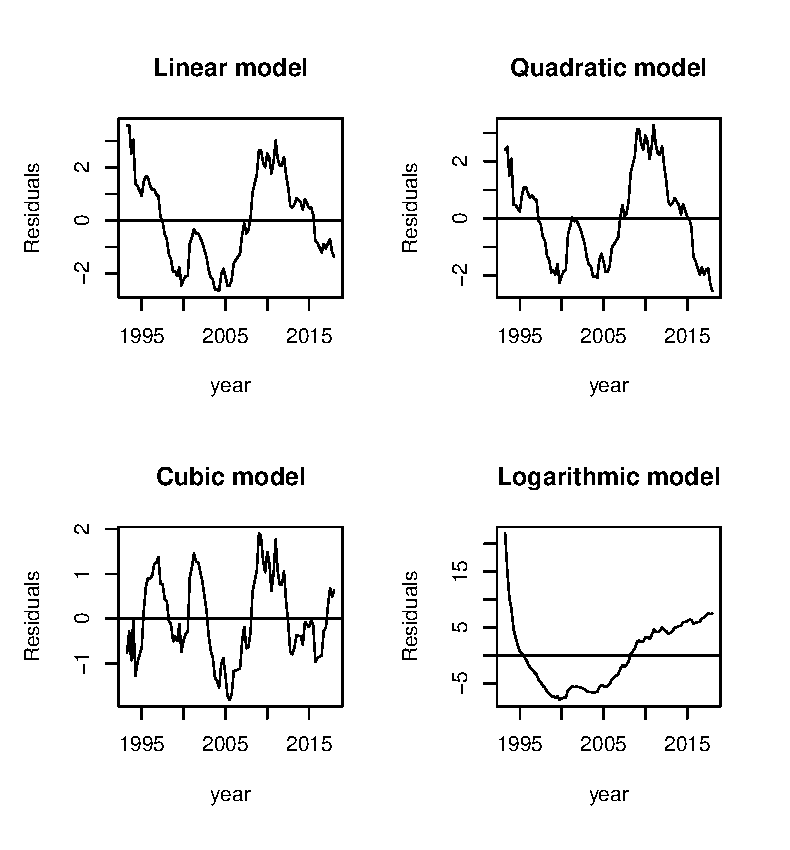
\includegraphics[width=0.8\textwidth]{resid_polynomials}
    \caption{Residuals of the fitted linear, quadratic, cubic and logarithmic model}
    \label{fig:resid_polynomials}
\end{figure}

Nevertheless, even though there is evidently a highly significant polynomial trend in the Swiss rent index series, that doesn't mean necessarily that its residual time series are stationary.
Unfortunately that happened as we can see from the four noise sequences in \cref{fig:resid_polynomials}.
The series wander up and down for quite some periods, meaning that the basic properties of stationary processes, time-independent expectation and constant variance over time are not fullfilled here \cite[p.~49]{bd02}.
Since we can already be sure from the residual plots that trend elimination by fitting polynomial models doesn't help to obtain a stationary series, we will not show further diagnostics on these and continue by trying to eliminate the trend by differencing.\footnote{Since the residual plots show strong time-depending covariances, by consequence the plots of the sample auto-correlation function (ACF) and partial auto-correlation function (PACF) of the fitted polynomial models showed likewise a strong auto-regressive process of order 1 (decreasing values in the ACF-plot and 1 spike in the PACF-plot with a lot of significant auto-correlations outside the 95-percent-confidence bounds of $+/-1.96/sqrt{n}$. This can be found in the appendix}. 


\subsection{Method 2: Trend elimination by differencing}
Since the fitted polynomial models didn't help to get a stationary time series we will try to eliminate the trend by differencing.
We will differentiate the data at different lags (1, 2, 3 and 4) in order to generate a noise sequence and hopefully get a stationary series \citep[p.~35]{bd02}.
Again we will show first the residual plots. Afterwards testing will be done by looking at the sample ACF and PACF as well as the Ljung-Box-Test for indepencence of the residuals and the Augmented Dickie-Fuller-Test for stationarity.


\subsubsection{Modelling the estimated noise sequences}

\begin{figure} 
    \centering
    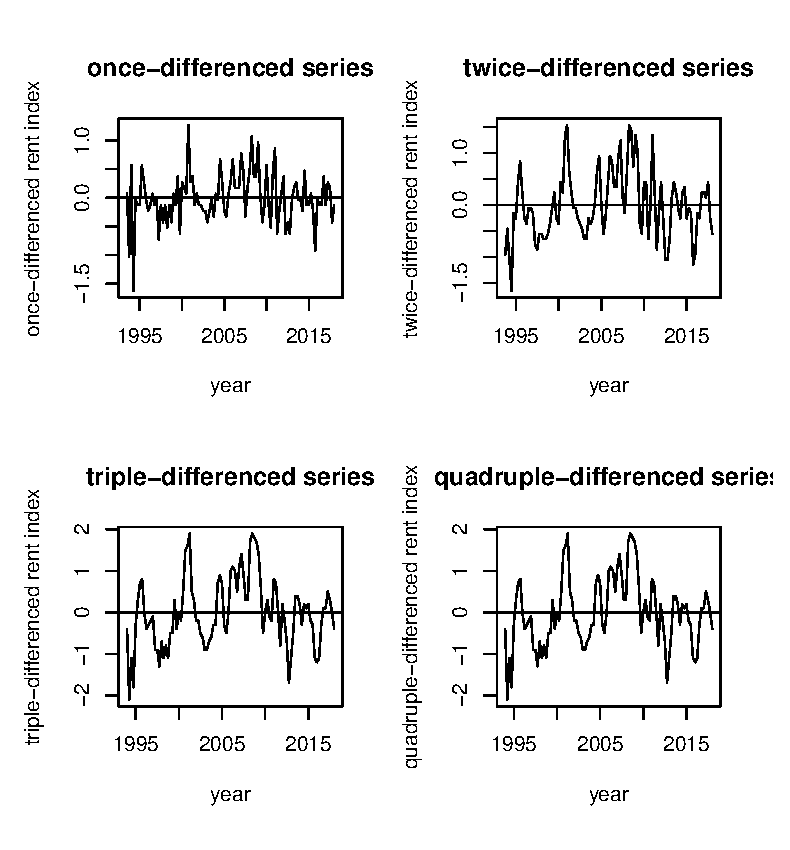
\includegraphics[width=0.8\textwidth]{resid_diff_all}
    \caption{Residuals of the differenced series}
    \label{fig:resid_diff_all}
\end{figure}

As we can see in the \cref{fig:resid_diff_all} the first two models look already quite promising in contrast to the residual time series above by polynomial trend elimination, showing here obviously time-independent noise sequences with presumably constant expectation and variance.

However, the lag1-differenced series show mostly patterns of a white-noise which is not what we intend since in case of a white-noise too much randomness is induced and the prediction quality becomes rather poor (expectation of all the predictions $X_{t+1}$, $X_{t+2}$, $X_{t+3}$ etc. would become zero in case of a mean-centered series).


\subsubsection{Testing the noise sequences}

We are going to test the estimated trends first visually, by looking on the sample ACF and the sample PACF, afterwards we are applying three diagnostic tests for stationarity and independence of the observations, respectively:
The Ljung-Box-Test \citep{LjungBox78} for independence as well as the Augmented Dickie-Fuller-Test for stationarity \citep{adf}.

As we can see in \cref{fig:diff12_acf_pacf}) the white-noise of the lag1-differenced series is confirmed by the sample ACF where all lags up to 40 fall within the bounds of $+/-1.96/sqrt{n}$ \cite[p.~39]{bd02}.
This underlines that the lag1-differenced series is to versatile and contains too much randomness in order to do good predictions.

\begin{figure} [ht]
    \centering
    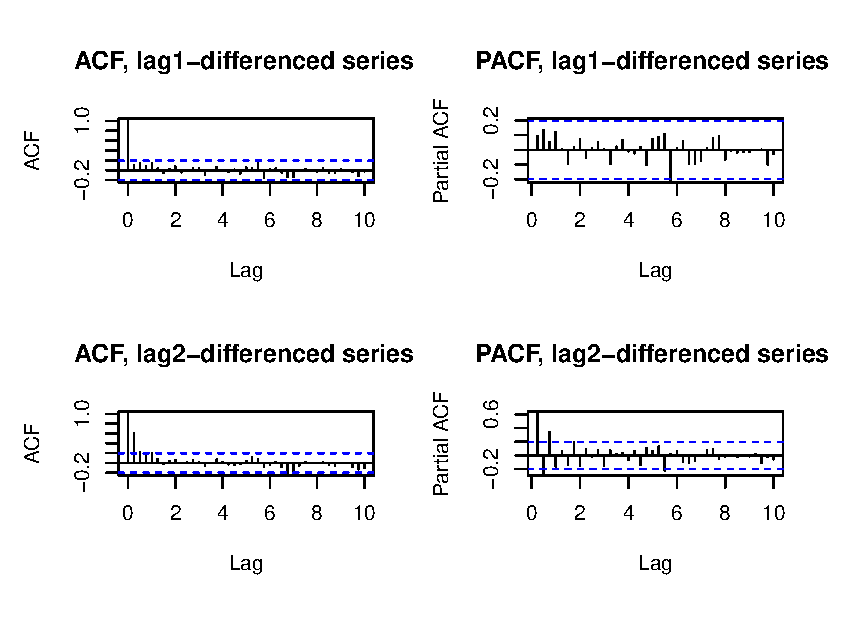
\includegraphics[width=1\textwidth]{diff12_acf_pacf}
    \caption{sample auto-correlation and partial auto-correlation function of the lag1- and lag2- differenced series}
    \label{fig:diff12_acf_pacf}
\end{figure}

In contrast, the sample ACF of the lag2-differenced model doesn't indicate a white-noise: there is at least a highly significant at lag1 and the following three lags are touching the $\pm 1.96 / \sqrt{n}$ - 95percent-confidence-bounds, followed by no more significant bars which die out quickly.
This is a good sign, meaning that on one hand we have at least correlation at lag 1 which is needed to do prediction, on the other hand the covariances seem obviously not too large to be considered time-dependant and therefore we can assume a stationary series here.

\begin{center}
\begin{tabular}{c|cccc}
    differentiation  & lag1 & lag2 & lag3 & lag4 \\
    \hline 
    \makecell{p-value Ljung-Box-Test\\($H_0$: White-noise)} & 0.35 & 0.00 & 0.00 & 0.00\\
    \makecell{p-value Augmented Dickie-Fuller-Test\\($H_0$: Non-Stationarity)} & 0.01 & 0.05 & 0.11 & 0.42\\
    \label{tab:overview_diffs}
\end{tabular}
\end{center}

From the tests overview in \cref{tab:overview_diffs} we can see for the lag1-differenced series a p-value of 0.35 for the Ljung-Box-Test.
That was to be expected, meaning that we cannot reject the Hypothesis $H_0$ that there is independence between the observations \citep{LjungBox78} and therefore confirming the white-noise structure in the lag1-differenced series. \\
In contrast again, the Ljung-Box-Test for the lag2-differenced series rejects the $H_0$ of independence which is a pleasant result giving us the sureness that there is no white-noise in the lag2-differenced series.\\
The Augmented Dickie-Fuller-Test suggest for the lag1- as well as for the lag2-differenced trend elimination a stationary time series (p-values < 0.05).\\
That is a very good result and we can finally conclude to stick with the lag2-differentiation in order to transform our data, since the lag1-differenced series is characterized by too much randomness and white-noise and the lag3- and lag4-differenced series show too large covariances (time-dependence/non-stationarity, indicated by a p-value of the ADF-Test by 0.11 and 0.42, respectively.\\
Finally we center our transformed data by subtracting the mean so that they are prepared fit and test ARMA-models.


% ------------------------------------------------------------------------

\section{Fitting and Testing the Model}
\label{sec:FitTestModel}

\subsection{Order and model selection}

From the sample ACF and PACF (\cref{fig:diff12_acf_pacf}) of our lag2-differenced series we can see in the ACF-plot a highly significant spike at the first auto-correlation $\hat{\rho_1}$ and the following bars dying out quickly, lying inside the 95percent - confidence – bounds.
The combined view of the PACF-plot with its exponentially decreasing patterns (in absolute values) and the 1 spike in the ACF-plot let us suggest an MA(1)-model could fit our data well.\\
However, since we are operating with only 100 observations, one can not exclude that there could be underlying exponentially decreasing patterns in the ACF plot as well since the bars die out so quickly.
Is this the case, then an exponential decrease (in absolute values) in both ACF and PACF plot would rather suggest an ARMA-model.

\begin{figure}
    \centering
    \includegraphics[width=0.5\textwidth]{aicc_matrix}
    \caption{AICC Matrix}
    \label{fig:aicc_matrix}
\end{figure}

Hence, according to the ACF and PACF plots it looks primarily like an MA(1)-process, but we cannot reject fore sure that it could be an ARMA-process as well, therefore AICC\footnote{
    The lower the AICC-value the better the model's performance \citep{aic86}.
} we compare as well AICC-values for ARMA-models with different orders of p and q\footnote{
    p indicates the order of the auto-regressive part and q the order of the moving-average part.
    Its coefficient are generally noted as $phi$ (AR-part) and $theta$ (MA-part).} in order to select our model.\\
From the AICC-Matrix (\cref{fig:aicc_matrix}) we can see that an MA(1)-model gives us the lowest AICC-value which means this model is supposed to perform best. That confirms our guess from the sample ACF/PACF plots.
However, we are also going to fit an ARMA(1,1) and an ARMA(1,2) model, because both of them showed as well very low AICC-values (see AICC-Matrix in figure).\footnote{
    Estimations by the autofit()-function of the "itsmr" package of R by \cite{R_itsmr} suggest as well an MA(1)-model as best model with a very similar estimate for $\theta_1$ and very close AICC.
    Furthermore ARMA(1,1) and ARMA(1,2) are also suggested by the autofit()-function showing very low AICC-values.
    This can be seen as a succesful robustness check in terms of order selection of p and q.
}

We now estimate coefficients (\cite[p.~83]{bd02}) for these three model candidates by the arima()-function of the R-package "stats" \citep{R_core}.


\begin{align*}
   \text{MA(1)-model: } X_t = Z_t + \theta_1 Z_{t-1}
    & \text{where ${Z_t} \sim WN(0,\sigma^2)$} 
\end{align*}

with the estimated coefficient and the corresponding standard error (in brackets):
%
% Hier mal 2 variante: kompakt und lang
%
% Version kompakt
\begin{align*}
    \hat{\theta}_1  &= \num{ 1.0000 \pm 0.0651}  &  \hat{\sigma}^2  &= \num{ 0.1847 }
\end{align*}


\begin{align*}
    \text{ARMA(1,1)-model: }X_t - \phi_1 X_{t-1} &= Z_t + \theta_1 Z_{t-1}
    & \text{where ${Z_t} \sim WN(0,\sigma^2)$} 
\end{align*}

with the estimated coefficients and the corresponding standard errors (in brackets)
%
% Hier mal 2 variante: kompakt und lang
%
% Version kompakt
\begin{align*}
    \hat{\phi}_1    &= \num{ 0.1336 \pm 0.1071}  &  \hat{\theta}_1  &= \num{ 0.9786 \pm 0.0784}  &  \hat{\sigma}^2  &= \num{ 0.1838 }
\end{align*}


\begin{align*}
    \text{ARMA(1,2)-model: }X_t - \phi_1 X_{t-1} &= Z_t + \theta_1 Z_{t-1} + \theta_2 Z_{t-2}
    & \text{where ${Z_t} \sim WN(0,\sigma^2)$}    
\end{align*}

with the estimated coefficients and the corresponding standard errors (in brackets):
%
% Hier mal 2 variante: kompakt und lang
%
% Version kompakt
\begin{align*}
    \hat{\phi}_1    &= \num{ 0.7974 \pm 0.2055}  &  \hat{\theta}_1  &= \num{ 0.3092 \pm 0.2528} &
    \hat{\theta}_2  &= \num{-0.6685 \pm 0.2583}  &  \hat{\sigma}^2  &= \num{ 0.1793 }  
\end{align*}

\TODO{clean up the mess above, write it into fliesstext maybe like the following?}

The ARMA(1,2)-model
    \( X_t - \phi_1 X_{t-1} = Z_t + \theta_1 Z_{t-1} + \theta_2 Z_{t-2} \),
    where \( {Z_t} \sim WN(0,\sigma^2) \)
    and with the estimated coefficients and the corresponding standard errors of
    \(\hat{\phi}_1 = \num{ 0.80 \pm 0.21} \),
    \( \hat{\theta}_1  = \num{ 0.31 \pm 0.26} \),
    \( \hat{\theta}_2 = \num{-0.67 \pm 0.26} \) and
    \( \hat{\sigma}^2 = \num{ 0.18 } \).


First we can see that ARMA(1,1)-model is not supposed to be a good model. Its estimated $\hat{\phi}_1=0.13$ is not significant, since its standard error of 0.11 is nearly as high as the coefficient.\\
In contrast, an ARMA(1,2)-model looks quite promising. First, its AR-term would become significant, taking a value of $\hat{\phi}_1=0.79$ and second, we can derive evidence for the estimates of the two MA-terms by considering an additional MA-term. An ARMA(1,3)'s $\hat{\theta}_1 = 0.35$ and $\hat{\theta}_2= -0.60$ would not differ a lot from the ARMA(1,2)'s $\hat{\theta}_1 = 0.31$ and $\hat{\theta}_2 = -0.67$. Furthermore an additional MA-term $\hat{\theta}_3 = 0.05$ is not significant since it would be close to 0 with a large standard error, indicating that the explanatory power by adding a third $\hat{\theta}$- term would be rather poor, indicating that an ARMA(1,3) is overfitted model. Therefore emphasizing that a moving average of order 2 would be a suitable choice.
But we have to note that $\hat{\theta}_1$ and $\hat{\theta}_2$ are rather small compared to their standard errors.
$\hat{\theta}_1$ is only slightly larger than its standard deviation.
$\hat{\theta}_2$ is 2.5 times larger.
\\
The MA(1) is also performing very well, however with a value of 1.00 $\hat{\theta}_1$ implies a unit root on the moving-average polynomial. But that is only a minor issue in comparison to unit roots on the autoregressive polynomial \cite[p.~42--83]{bd02} which is not the case here. Therefore we want to stick with the MA(1) and ARMA(1,2) as our candidate models.



% % Alles in einer spalte
% \begin{align*}
%     \hat{\phi}_1    &= \num{ 0.7974 \pm 0.2055} \\
%     \hat{\theta}_1  &= \num{ 0.3092 \pm 0.2528} \\
%     \hat{\theta}_2  &= \num{-0.6685 \pm 0.2583} \\
%     \hat{\sigma}^2} &= \num{ 0.1793 }
% \end{align*}





\subsection{Diagnostics of the model}

To check the validity of our candidate models we apply the following diagnostics:\\
First, we plot the rescaled residuals and verify that there is not some obvious dependence, trend or else. We should see a white-noise if the model is valid.\\
Second, we have a look at the ACF of the rescaled residuals.
Since we are supposed to have a white-noise approximately 95percent of the sample-autocorrelations rhohhat should be inside the bounds $\pm 1.96 / \sqrt{n}$. \\
Third we use the Ljung-Box Test \citep{LjungBox78} to validate or not that the residuals are white-noise by showing p-values for each lag \TODO{cite page 5 Lecture notes 11}.

\begin{figure}
    \centering
    \includegraphics[width=0.5\textwidth]{ts_diag_ma_1}
    \caption{MA(1)-Model: Standardized Residuals, Auto-correlation function of the Residuals and the p-values for the Ljung-Box-Test at each lag}
    \label{fig:ts_diag_ma_1}
\end{figure}
\begin{figure}
    \centering
    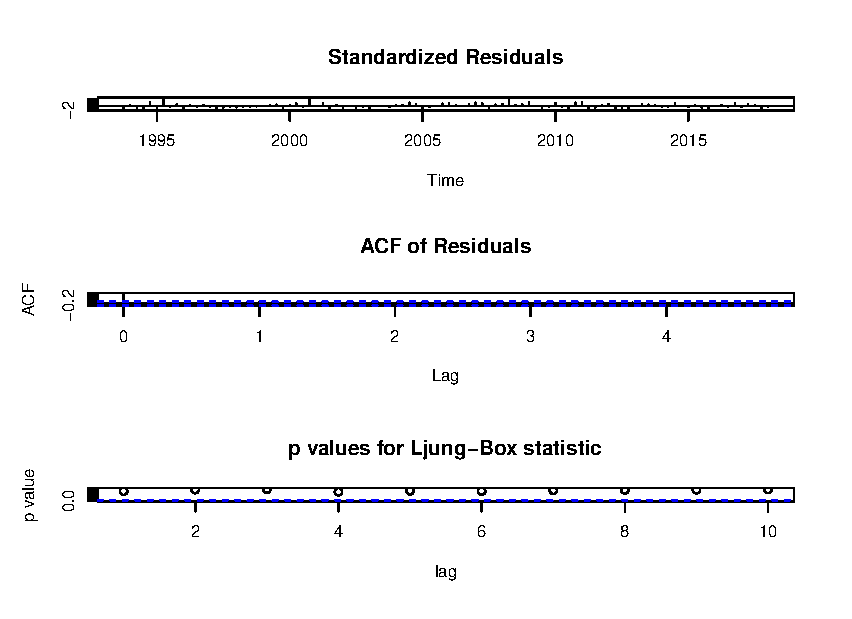
\includegraphics[width=0.5\textwidth]{ts_diag_arma_1_2}
    \caption{ARMA(1,2)-Model: Standardized Residuals, Auto-correlation function of the Residuals and the p-values for the Ljung-Box-Test at each lag}
    \label{fig:ts_diag_arma_1_2}
\end{figure}

We are visualizing these diagnostics by using the tsdiag() function from the "stats" R-Package \TODO{\citation{R Core Team}}.
The following \cref{fig:ts_diag_ma_1} and \cref{fig:ts_diag_arma_1_2} show these three diagnostics for both of our candidate models, the MA(1) and the ARMA(1,2).
We can see that the standardized residuals are supposed to be white-noise in both cases.
In addition, from the ACF of the rescaled residuals we can see that not a single bar (out of 20) lies outside the bounds bounds $\pm 1.96 / \sqrt{n}$.
And from the Ljung-Box-Tests we can see that the p-value is larger than 5 percent for each lag for each model, meaning that we cannot reject the Hypothesis H0 that these residuals are a white-noise. So both models MA(1) and ARMA(1,2) would be valid and could be used for forecasting.


% ------------------------------------------------------------------------

\section{Prediction of future values}

In this section we want to predict future values on the base of our fitted MA(1)- and ARMA(1,2)-models.
We will do that by first forecasting our transformed (lag2-differenced) series.
Afterwards we will do a retransformation into the initial time series and predict its future values.
In addition, we will give 95 percent confidence bands in case of normally distributed residuals.

\begin{figure}
    \centering
    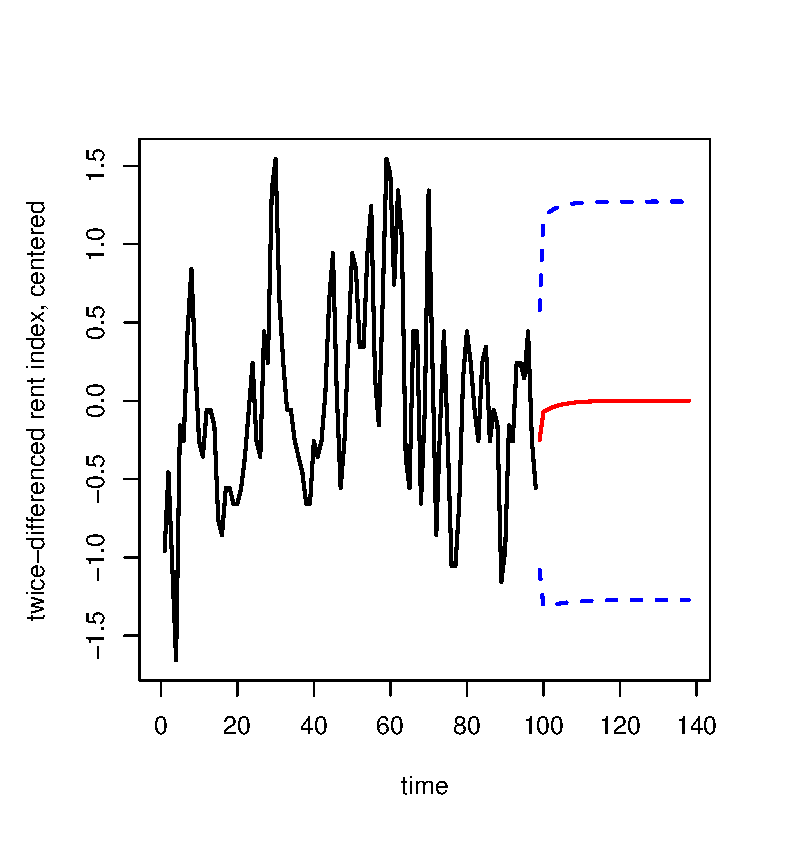
\includegraphics[width=0.5\textwidth]{pred_transformed_series}
    \caption{Prediction and Confidence Bands for the lag2-differenced Series, MA(1) and ARMA(1,2)}
    \label{fig:pred_transformed_series}
\end{figure}

From \cref{fig:pred_transformed_series} we can see the prediction of a process of adaptation to the zero-mean for the next 8 quarters.
Both models show a prediction tendency to the zero-mean which is nothing surprising for a mean-centered stationary time series. However, the ARMA(1,2)-model shows a smoother and slower adaptation process to the zero-mean, representing a more reasonable forecast than the MA(1). In comparison the MA(1)-model would only predict for $X_{n+1}$ a value different from the zero-mean. For all the following $X_{n+2}$,$X_{n+3}$ etc. MA(1) it would abruptly predict zero-mean. Hence, the MA(1)-model's prediction power is not that high and beside the prediction of $X_{n+1}$, wouldn't even differ from predictions based on a pure white noise sequence.  \\
The quite large 95-percent confidence bands are not that surprising in a strongly differenced series as we have here. Differenced series  can contain quite large amplitudes as we can.\footnote{
    The indication of confidence bands is weakly justified here since the series’ residuals are successfully tested for normal distribution by the Shapiro-Wilk-Normality Test. \TODO{missing sentence} showed a p-value of 0.12 in case of MA(1) and 0.07 in case of ARMA(1,2), meaning that the hypothesis H0 of normal distribution can slightly not be rejected \citep{shapiro}.
    However, a quantile-quantile-plot showed patterns of normal distribution for the close-to-mean observations but slightly heavier tails compared to a true normal distribution.
    Therefore interpretations of confidence bands are to be handled with care.
}
However, it would be desirable to reduce the variance and by consequence the confidence bands by increasing the number of observations. \\
\begin{figure}
    \centering
    \includegraphics[width=0.5\textwidth]{pred_initial_series}
    \caption{Prediction and Confidence Bands for the initial series, MA(1) and ARMA(1,2)}
    \label{fig:pred_initial_series}
\end{figure}
Having a look at the predictions for the initial time series\footnote{The prediction of the initial series bases on retransformation of the lag2-differenced series into the initial series.} \cref{fig:pred_initial_series} we can intuitively see that the predictions in both models MA(1) and ARMA(1,2) are reasonable, indicating a strongly monotonic trend in the future. However, due to the smoother and slower adaptation process to the expectation of the mean we definitely want to stick with the ARMA(1,2)-model as our favourite model.


% ------------------------------------------------------------------------

\section{Discussion}

\TODO{Discuss your results, the strengths and the limitations of your own analysis.}
The strength of the project lies in the forecast of the ARMA(1,2)-model which gives us a reasonable monotonically increasing prediction which smoothly adapts to the expected mean within the upcoming few quarters. \\
The difficulty of this project was the problem to get the data transformed into a stationary timeseries in a way that the residuals don't show too much randomness (no white-noise) on the one hand, and on the other hand that we get a few significant auto-correlations $\hat{rho}$ in order to do good predictions based upon past observations. \\Since the initial time series was strongly monotonically increasing and therefore likewise strongly positively auto-correlated, achieving a stationary series became a hard task: first, trend elimination by polynomial trend fitting was not possible because of the heavy auto-covariances, second lag1-differencing turned out to be not applicable neither and causing the opposite problem, meaning too much white noise. \\
    Lag2-differencing finally did the job. But that is not a totally satisfying transformation since the series was definitely not seasonal as proven in the section 3, and lag2-differentiation normally is used to get rid of a seasonal component with d=2. 
    \\Furthermore the MA(1)-model turned out to show a minor issue due to a unit root in the moving-average polynomial (estimated $\hat{\theta_1} = 1.00$) which could possibly indicate an overdifferencing according to \cite[~p.194]{bd02}. When a root of the process is close to the unit circle the asymptotic distribution of the maximum likelihood can be quite inadequate \citep{davidson81}. However, other authors have shown that an estimation by maximum likelihood differ only slightly from estimations by other methods as \citep{davisdunsmuir96} have shown and that $\hat{\theta_1}$ close to 1 is not that big of a deal and it is certainly from minor importancein contrast to a unit root on the autoregressive polynomial\citep{plosser77}. \\
To conclude, the choice of the correct data transformation was the dilemma between a lag1-differentiation which would have lead to an undesirable white-noise sequence and a lag4-differentiation which was not anymore stationary (p-value of augmented Dickie-Fuller-Test of 0.42 (editor's comment: alternative hypothesis is stationarity \citep{adf}). In between those two extreme options only the lag2-differentiation was stationary on the one hand and allowed for better prediction power thanks to at least one significant autocorrelation. \\
Furthermore, our model of choice, the ARMA(1,2) process, does in fact not show a unit root on the moving average polynomial (which would not be that severe as we evoked above), but we have to note that its $\hat{\theta_1}$-coefficient lacks of reliability since its standard error was not that small. The relatively small n of 100 observations was one reason for the relatively high standard error. Hence, for further predictions on the rent index a larger number of observations would be desirable.



% ------------------------------------------------------------------------

\section{Conclusion}

Both of the suggested candidate models, the MA(1)- and the ARMA(1,2)-model turned out to be good models in order to predict our data. Both of them passed the diagnostics of independent residuals very well and both are predicting a reasonable, strongly monotonic trend in the future. However, due to the smoother and slower adaptation process to the expected of the mean we decided to stick with the ARMA(1,2)-model.
\\
This smoothly adapting positive trend is more realistic and goes confirm not only with the long-lasting and consistently increasing trend in the past, but as well with hypothesis about the Swiss rent market development where expert predict a slight slow-down of the growth in rents but a still remaining positive (but slower increasing) trend \TODO{zitiere nzz oder so}. \\

Further analysis could be done on the data analysis by treating the two segments before and after the subprime crises (before and after the year 2009) in different ways, since they showed slightly different increasing patterns. One possibility could be, for instance, to try first to logarithmize the stronger increasing data from 1993 to 2009 and afterwards eager for a linear trend elimination or differencing transformation on the total of the data.  \\

Further improving work could be done, first of all on the transformation into a stationary time series. Normally, if one uses a lag2-differentiation this is suggesting a seasonal component. This was clearly not the case in our timeseries as tested in section 3. Therefore the transformation process into a stationary time series is not completely satisfying and could be certainly improved by finding other transformation methods, for instance to check as well for the Brockwell-Davis-Method \citep{bd02}. \\

Second, given the fact that the quite promising MA(1)-model (in terms of the ACF and PACF patterns as well as the lowest AICC) didn't turn out be an ideal choice because of the unit root detected in the moving average polynomial. Even though it is not a severe issue, it could be worth to test drawing inference in another way, meaning that the estimation of the $\theta$-coefficient shouldn't rely only on the maximum likelihood function, but to try alternative estimations which are less vulnerable to the asymptotic distribution of the maximum likelihood, for instance trying a locally best invariant unbiased (LBIU) approach \cite{davissong11}, and afterwards comparing the two different estimates. That could be worth a try, especially if we take into account that a simulated MA(1)-process with $\theta_1 = 1.00 $ (see \cref{fig:sim_ma_1_00} in the  \TODO{apeendix}) is indicating the model PACF to decrease much slower than the sample PACF, suggesting that a $\theta_1 = 1.00 $ is maybe overestimated and alternative estimation methods are justified. A simulated model with $\theta_1 = 0.5 $ for instance would look more like the sample ACF/PACF (see \cref{fig:sim_ma_1_05} in the \TODO{apeendix}).

\pagebreak

% ------------------------------------------------------------------------


\bibliography{bibliography/bibliography}
\pagebreak

% ------------------------------------------------------------------------
% ------------------------------------------------------------------------

\appendix

% ------------------------------------------------------------------------

\section{Tables}

\begin{figure} [htb!]
    \centering
    \includegraphics[width=0.7\textwidth]{summary_cubicmodel}
    \caption{summary statistics of the fitted cubic model}
    \label{fig:summary_cubicmodel}
\end{figure}

\begin{figure}
    \centering
    \includegraphics[width=0.7\textwidth]{summary_seasonmodel}
    \caption{summary statistics of the fitted seasonal model}
    \label{fig:summary_seasonmodel}
\end{figure}

\begin{figure}
\centering
\includegraphics[angle=0,
width=0.6\textwidth]{acf_pacf_linearmodel}
\caption{Sample Autocorrelation and Partial autocorrelation function of the linear model
\label{fig:acf_linearmodel}}
\end{figure}
\begin{figure}
\centering
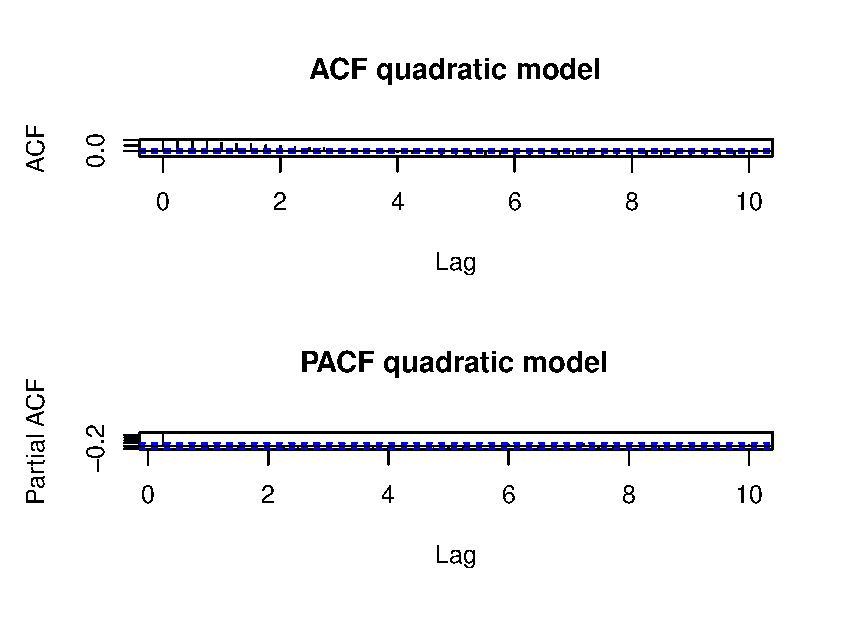
\includegraphics[angle=0,
width=0.6\textwidth]{acf_pacf_quadraticmodel}
\caption{Sample Autocorrelation and Partial autocorrelation function of the quadratic model
\label{fig:acf_quadraticmodel}}
\end{figure}
\begin{figure}
\centering
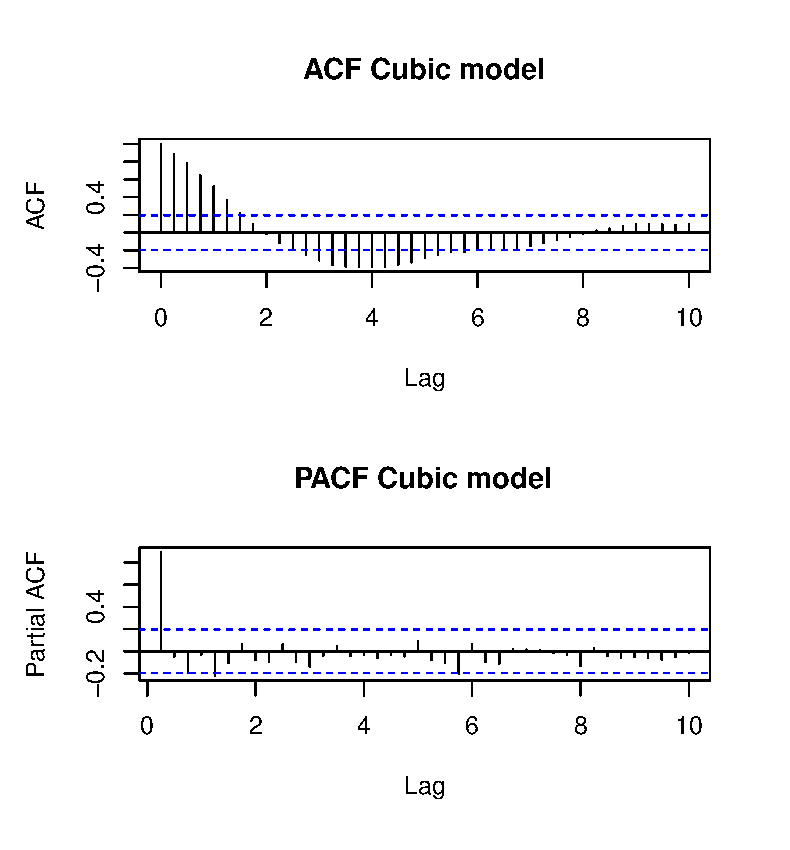
\includegraphics[angle=0,
width=0.6\textwidth]{acf_pacf_cubicmodel}
\caption{Sample Autocorrelation and Partial autocorrelation function of the cubic model
\label{fig:acf_cubicmodel}}
\end{figure}
\begin{figure}
\centering
\includegraphics[angle=0,
width=0.6\textwidth]{acf_pacf_logmodel}
\caption{Sample Autocorrelation and Partial autocorrelation function of the logarithmic model
\label{fig:acf_logmodel}}
\end{figure}


% ------------------------------------------------------------------------


\section{Simulations}
\begin{figure}
    \centering
    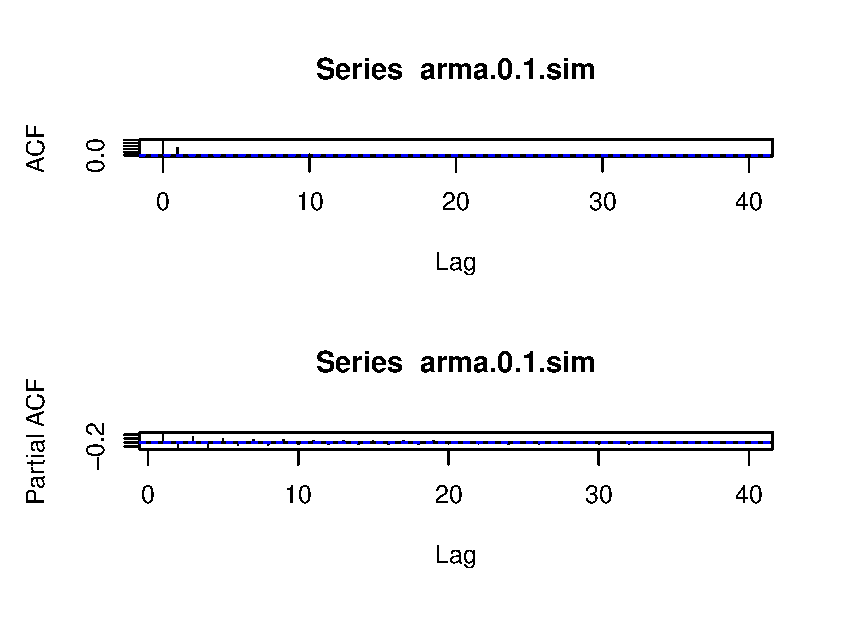
\includegraphics[width=0.7\textwidth]{sim_ma_1_00}
    \caption{model ACF and PACF of a simulated MA(1)-process with $\hat{\theta_1} = 1.00$ }
    \label{fig:sim_ma_1_00}
\end{figure}

\begin{figure}
    \centering
    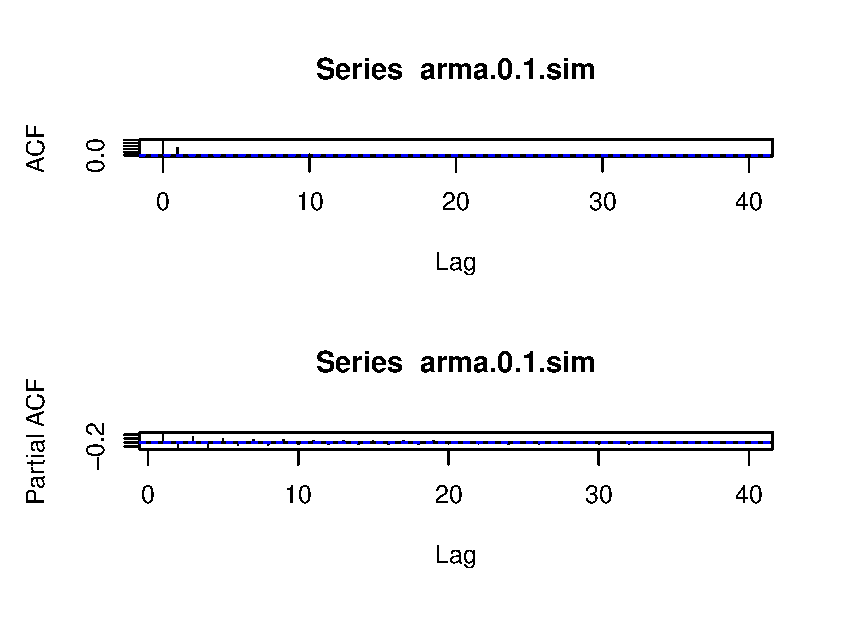
\includegraphics[width=0.7\textwidth]{sim_ma_1_00}
    \caption{model ACF and PACF of a simulated MA(1)-process with $\hat{\theta_1} = 0.5$ }
    \label{fig:sim_ma_1_05}
\end{figure}


\section{Cross-validation of the lag2-differenced series}

Cross-validation with a test data set considering only the last 35 of the 100 observations (see \cref{fig:diff2_testset} above) confirms furthermore the non-stationary character of the lag2-differenced-model 
Box.test(d2.indiceloyers.test, lag=2, type="Ljung-Box") p-value of 0.033 suggests the data are (time-)independent
adf.test(d2.indiceloyers.test, alternative = "stationary", k=2)  H0 of non-stationarity cannot be rejected which is not a problem, that could be due to lack of observations
kpss.test(d2.indiceloyers.test)  with a p-value>0.05 the test data seems to be stationary aswell
the data of the first period (1993 to 2009) lag2-differenced series show independent observations as well (see \cref{fig:diff2_test_train}), however we can see a slightly slower increase in the segment from 2009 to 2018 indicating that in the years from 1993 to 2009 the growth in rental prices was higher than in the years in the second's segment which begins from 2009. that can be explained by the big baisse in the early 90ies, starting from a lower initial point and better conjunctural perspectives the increase was stronger, whilst from 2009 on the growth in rental prices slowed down, which can be very well explained by the US subprime crises beginning in the year 2008 followed by a long-taking global recession.

\begin{figure}
    \centering
    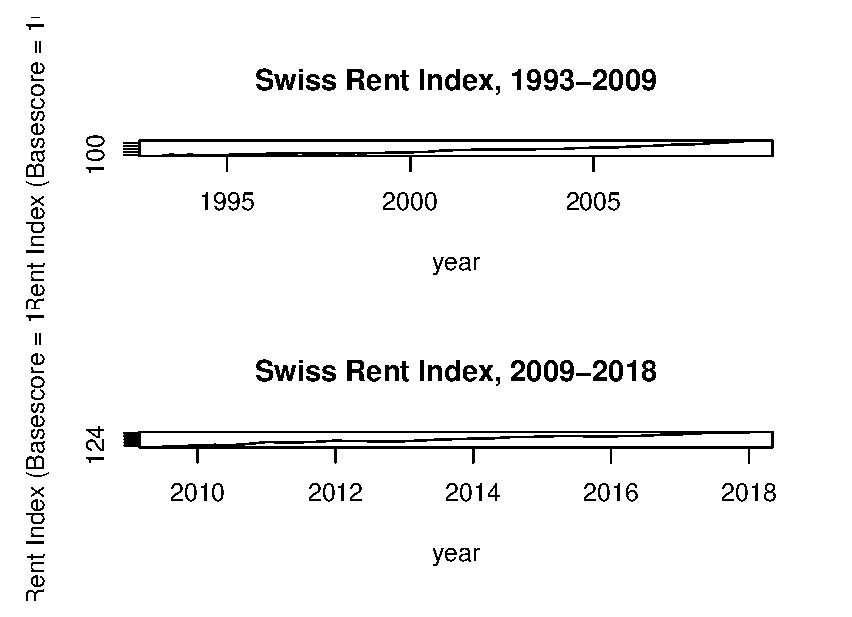
\includegraphics[width=0.8\textwidth]{diff2_test_train}
    \caption{mean-centered lag2-differenced series, periods from 1993 to 2009 and 2009 to 2018}
    \label{fig:diff2_test_train}
\end{figure}



\end{document} 
